\chapter{Implementacija i korisničko sučelje}


\section{Korištene tehnologije i alati}

\noindent Za komunikaciju tima korištene su aplikacije \underline{WhatsApp}\footnote{https://www.whatsapp.com/} i \underline{Discord}\footnote{https://discord.com}. Za izradu UML dijagrama korišten je \underline{Astah Professional}\footnote{http://astah.net/editions/professional}.

Za izradu dokumentacije korišten je \underline{LaTeX}\footnote{https://www.latex-project.org}, sustav za izradu dokumenata koji koristi markup jezik. Za upravljanje izvornim kodom korišten je \underline{Git}\footnote{https://git-scm.com/}. Repozitorij projekta dostupan je na platformi \underline{GitHub}\footnote{https://github.com}.

Za razvojna okruženja korišteni su \underline{Visual Studio Code}\footnote{https://visualstudio.microsoft.com/}. Visual Studio Code je integrirano razvojno okruženje (IDE) kompanije Microsoft. Koristi se za razvoj wen-stranica, web-aplikacija, web-usluga i mobilnih aplikacija. Za razvoj softvera koristi Windows API, Windows Forms, Windows Presentation Foundation, Windows Store i Microsoft Silverlight.

Za pisanje aplikacije korišten je \underline{Spring Boot}\footnote{https://spring.io/projects/spring-boot/}, framework za razvoj Java aplikacija, za razvoj backenda. Za razvoj frontenda korišten je \underline{React}\footnote{https://react.dev}, biblioteka za izgradnju sučelja u jeziku \underline{JavaScript}\footnote{https://www.javascript.com/}. Također je korišten \underline{TypeScript}\footnote{https://www.typescriptlang.org} kao nadrogradnja nad JavaScriptom. On poboljšava kvalitetu i održivost koda napisanog u JavaScriptu.

Baza podataka nalazi se na poslužitelju 

\eject


\section{Ispitivanje programskog rješenja}

%\textbf{\textit{dio 2. revizije}}\\

%\textit{U ovom poglavlju je potrebno opisati provedbu ispitivanja implementiranih funkcionalnosti na razini komponenti i na razini cijelog sustava s prikazom odabranih ispitnih slučajeva. Studenti trebaju ispitati temeljnu funkcionalnost i rubne uvjete.}


\subsection{Ispitivanje komponenti}
U procesu testiranja funkcionalnosti komponenti,  koristili smo popularni radni okvir \textit{JUnit}. Kako bi testiranje bilo izolirano, potrebno je simulirati komponente o kojima ovisi komponenta koju testiramo. U tu svrhu smo koristili programski okvir \textit{Mockito}. Ukupno smo implementirali sedam testirajućih metoda unutar tri testirajuće klase.

\vspace{1em}

U svrhu testiranja funkcionalnosti klase \textit{KorisnikController}, implementirali smo tri metode. Specifično, testirajuća metoda \ref{fig:test1} ima za cilj provjeriti ispravnost metode za registraciju novog korisnika kada su joj proslijeđeni valjani podaci za registraciju (ime, prezime, korisničko ime, lozinka, e-mail i uloga) te slika profila. Očekujemo da će rezultat testirane metode biti objekt tipa \textit{Korisnik}, koji će sadržavati točne podatke (prethodno proslijeđene) o novostvorenom korisniku.

\begin{figure}[H]
	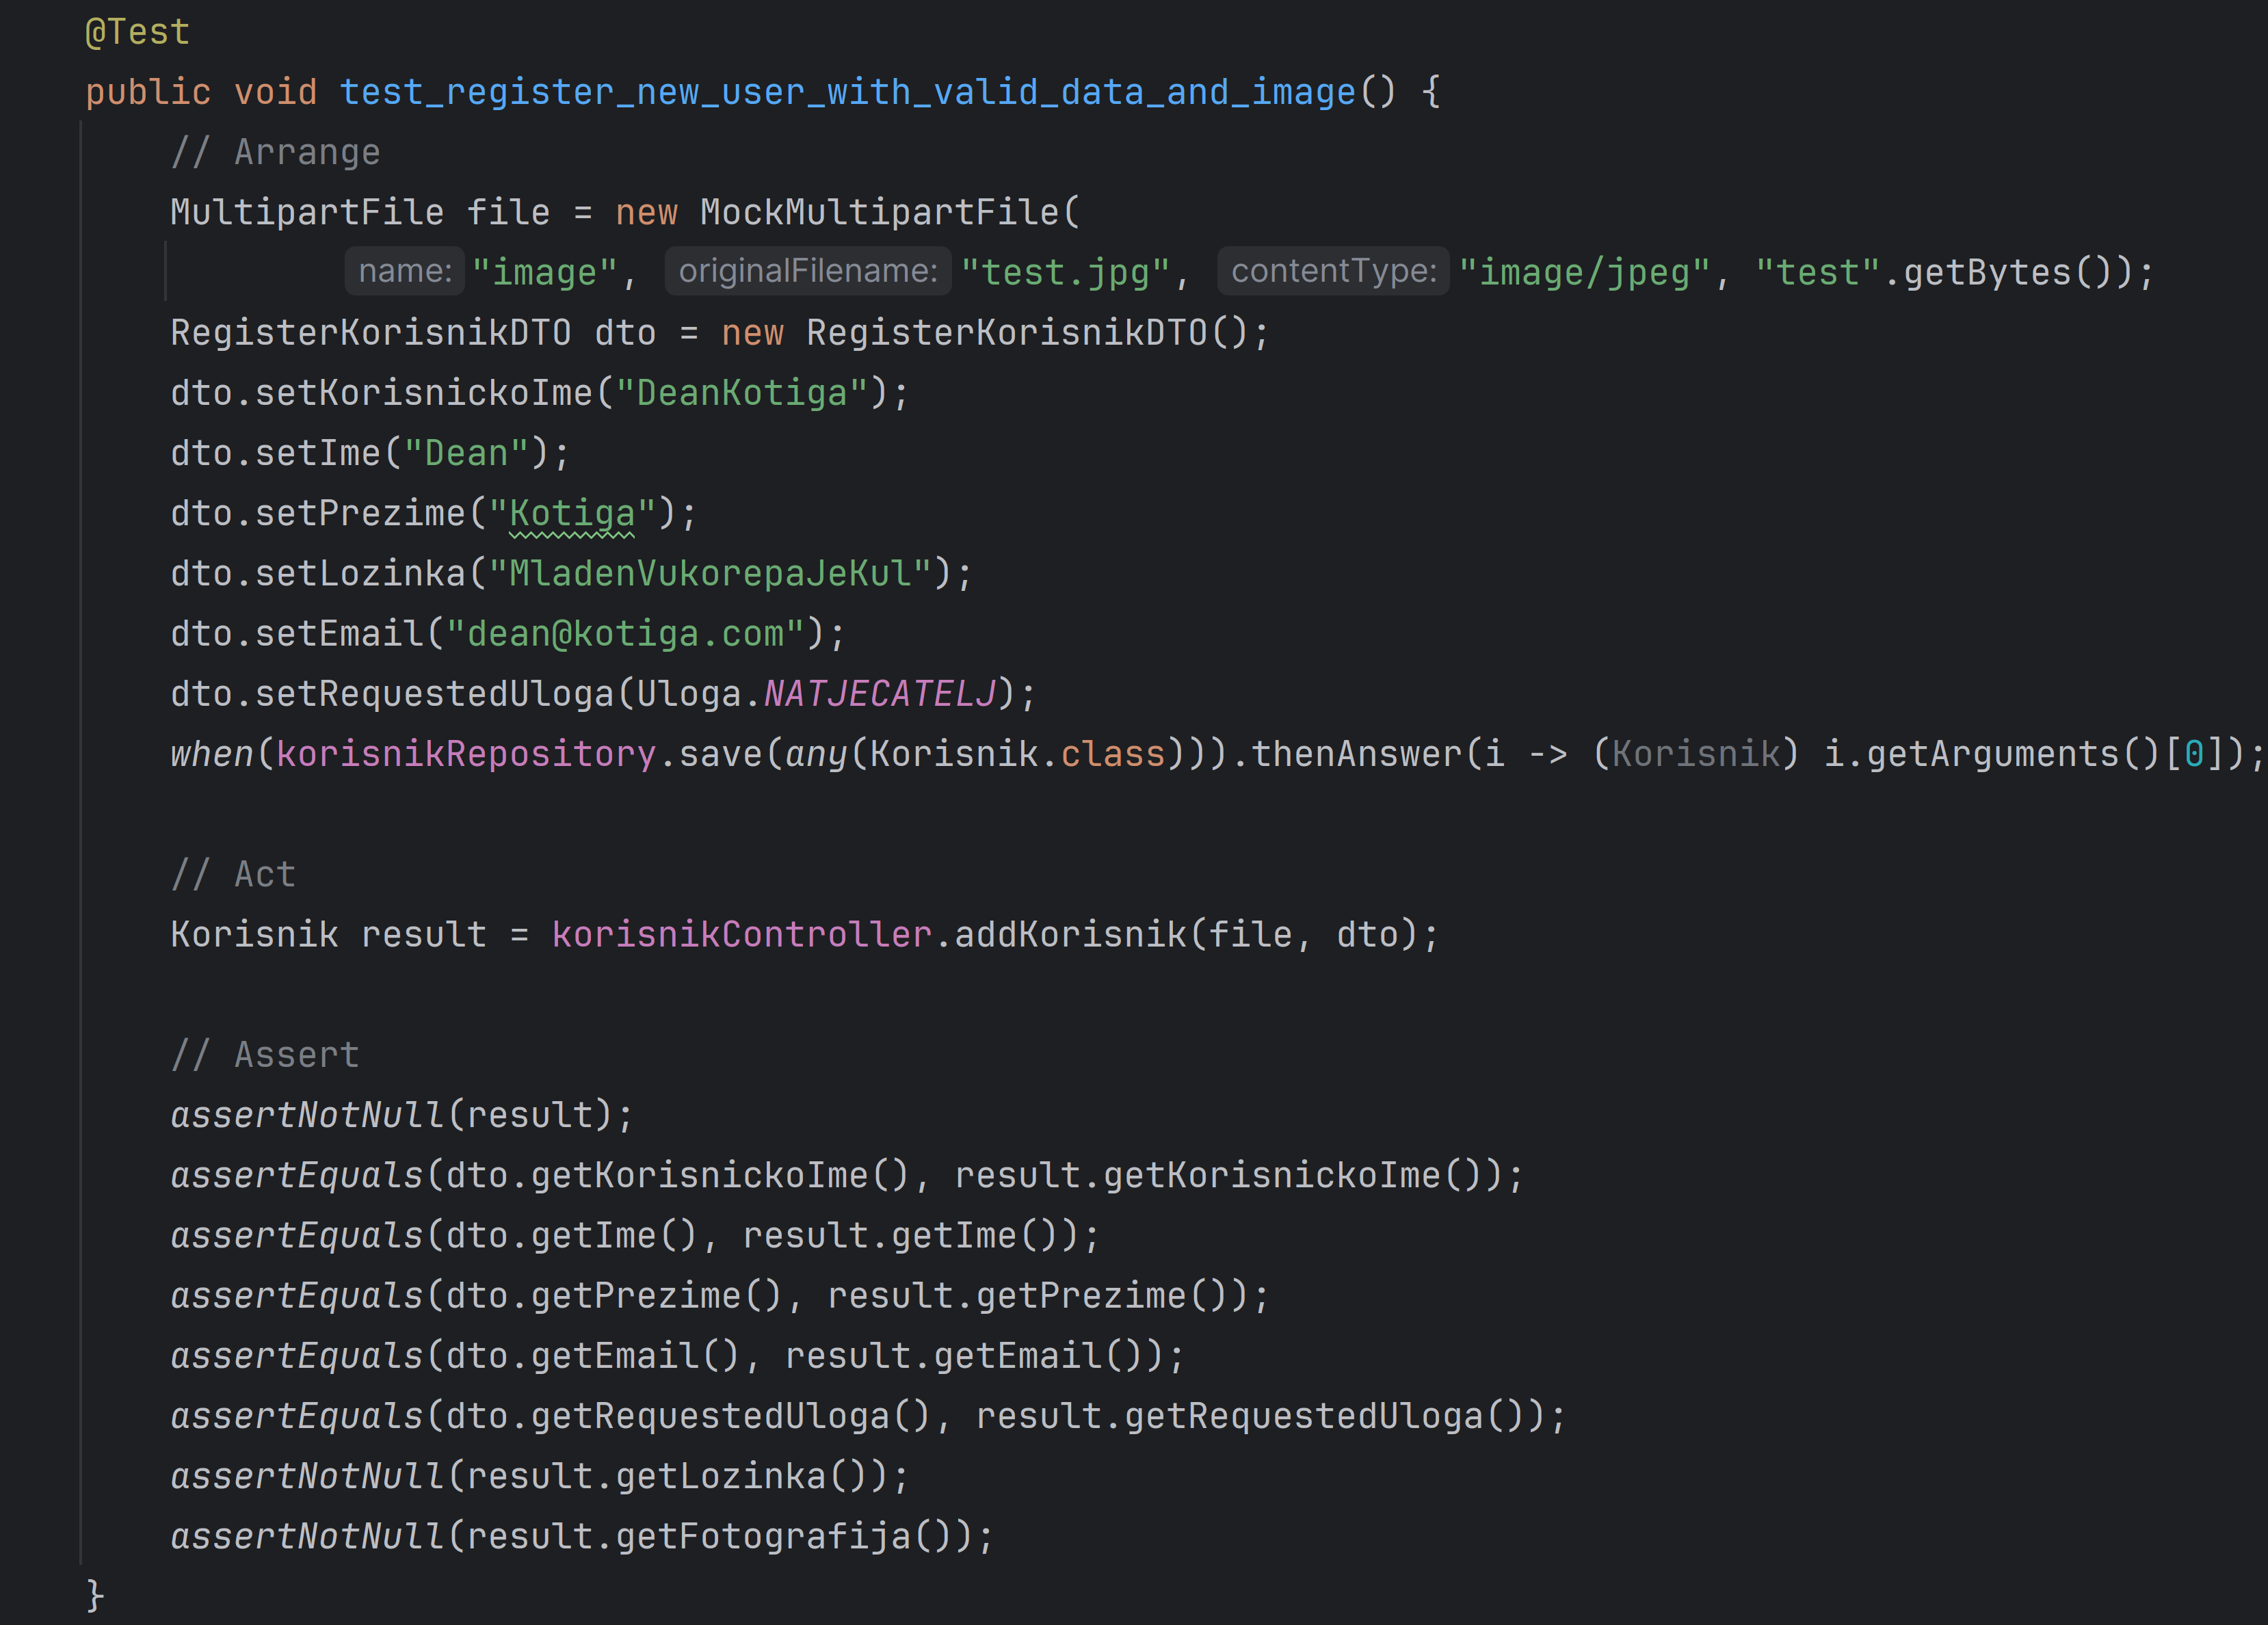
\includegraphics[scale=0.15]{slike/test1.png}
	\centering
	\caption{Testirajuća metoda - registracija korisnika}
	\label{fig:test1}
\end{figure}

Za razliku od prethodne, testirajuća metoda \ref{fig:test2} provjerava ispravnost iste metode u situaciji kada se pokuša dodati korisnik s korisničkim imenom koje je već zauzeto.  U ovome ispitnom slučaju se očekuje da će testirana metoda prepoznati ovu situaciju i shodno tome baciti očekivanu iznimku.

\begin{figure}[H]
	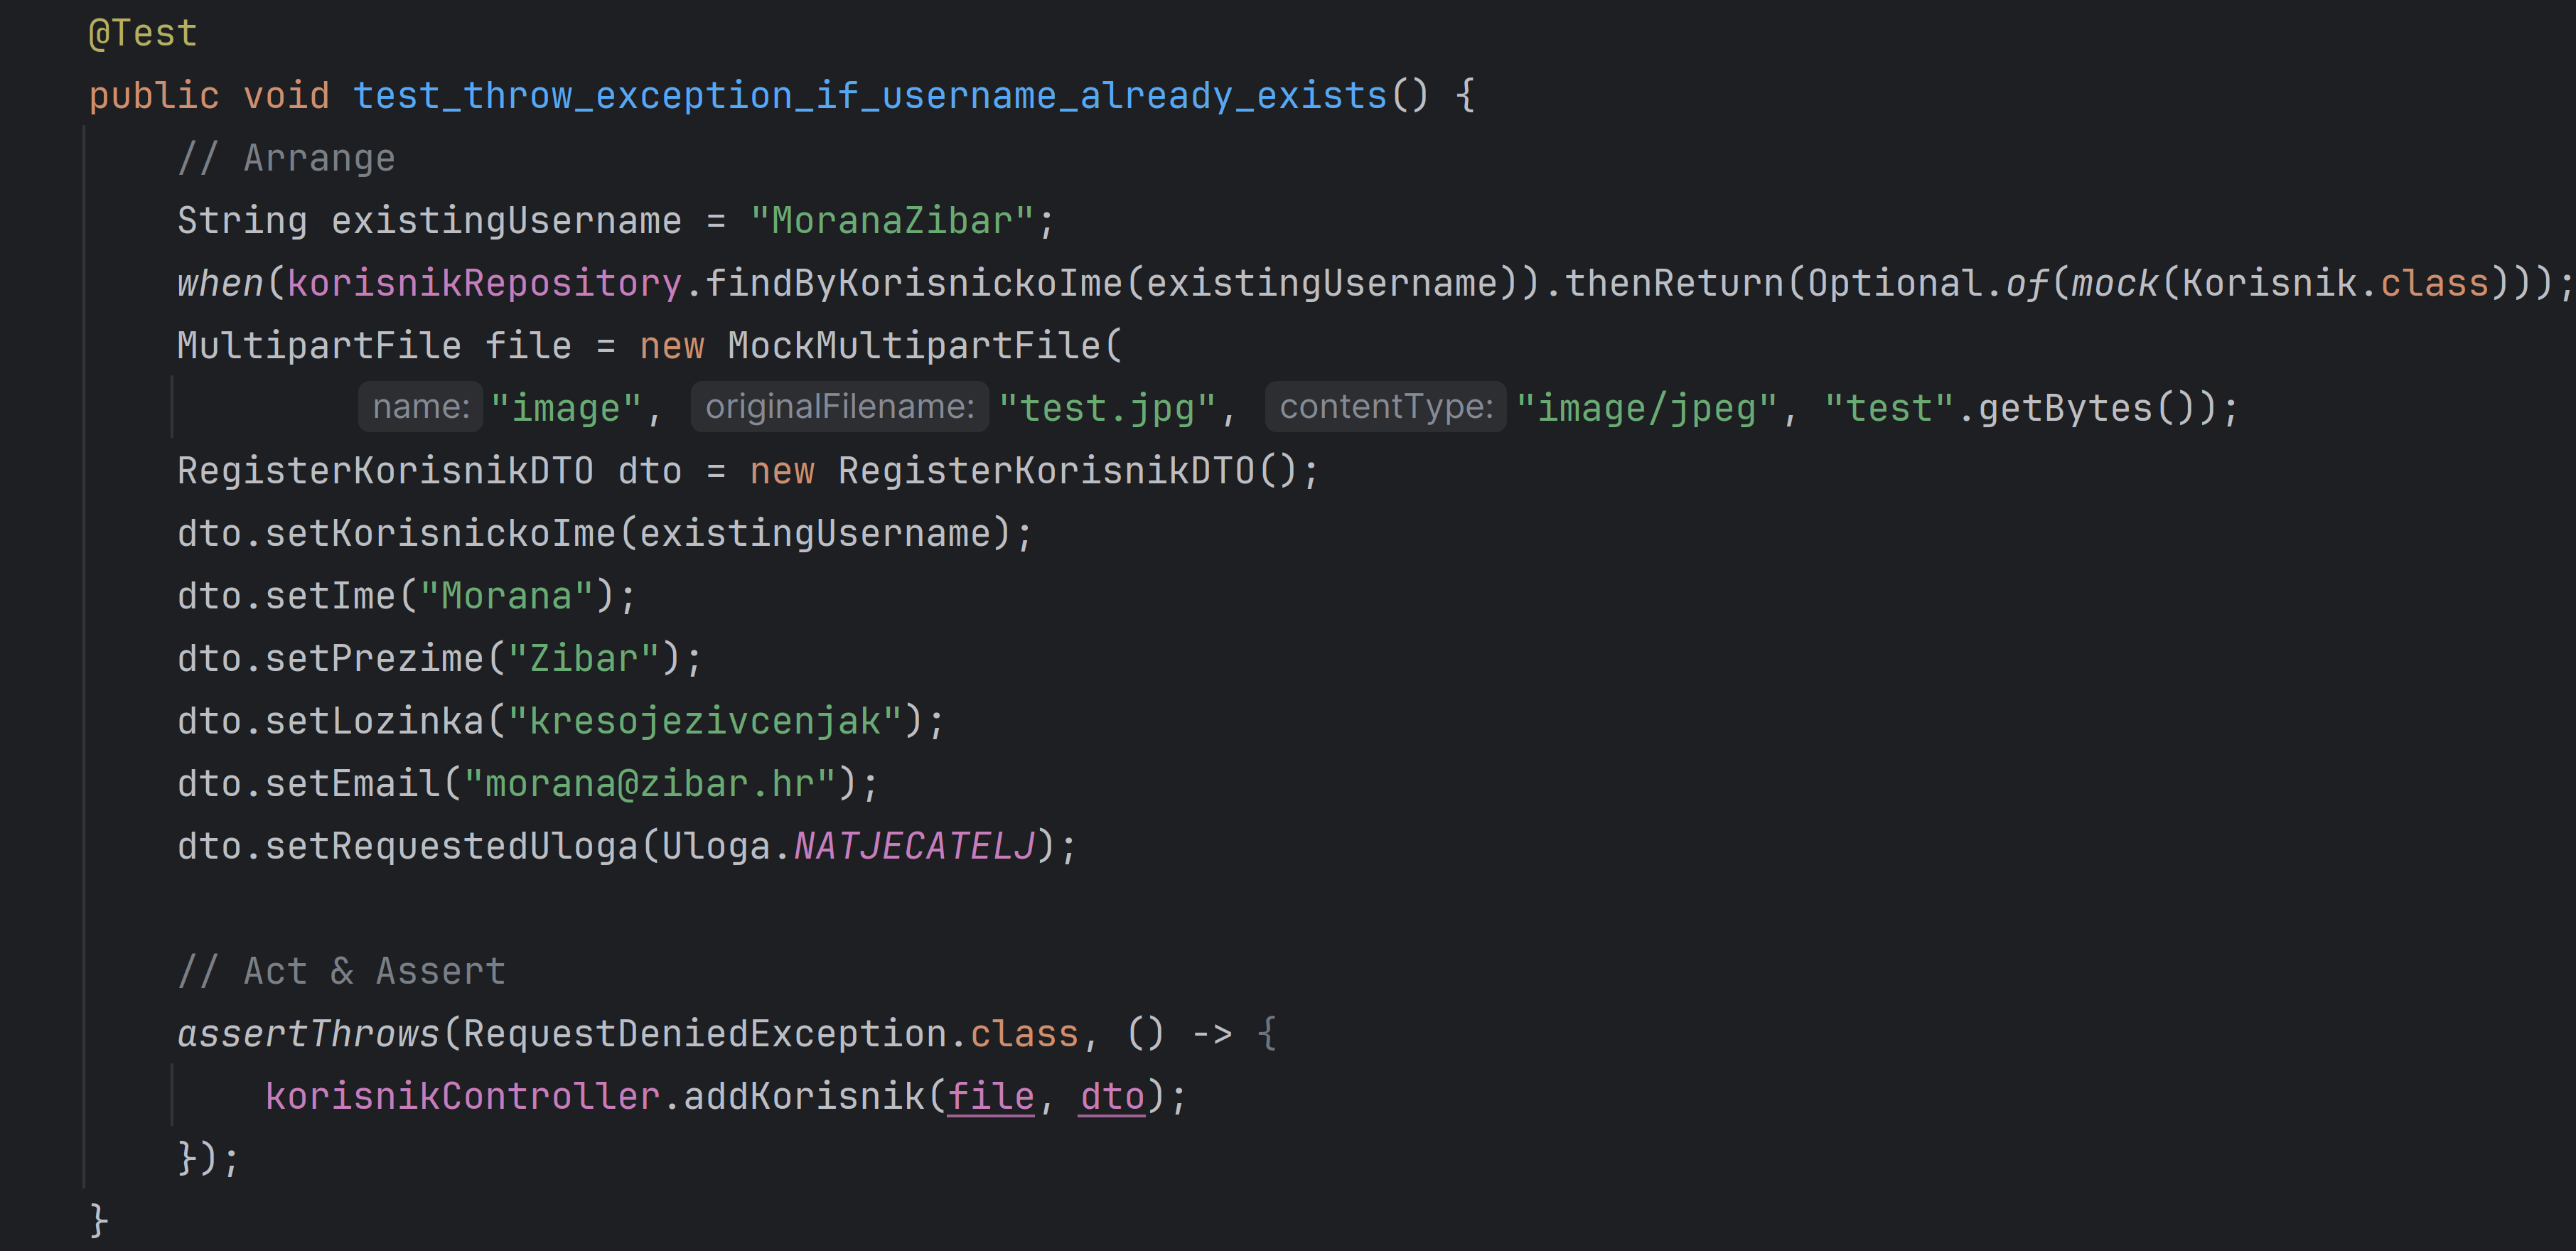
\includegraphics[scale=0.15]{slike/test2.png}
	\centering
	\caption{Testirajuća metoda - neuspješna registracija korisnika}
	\label{fig:test2}
\end{figure}

Posljednjim ispitnim slučajem \ref{fig:test3} za klasu \textit{KorisnikController} želimo verificirati  ispravnost metode za potvrdu zahtijevanih uloga korisnika od strane administratora. Očekuje se da će nakon uspješne potvrde testirana metoda, koja kao argument prima korisničko ime, vratiti HTTP odgovor sa statusom OK.

\begin{figure}[H]
	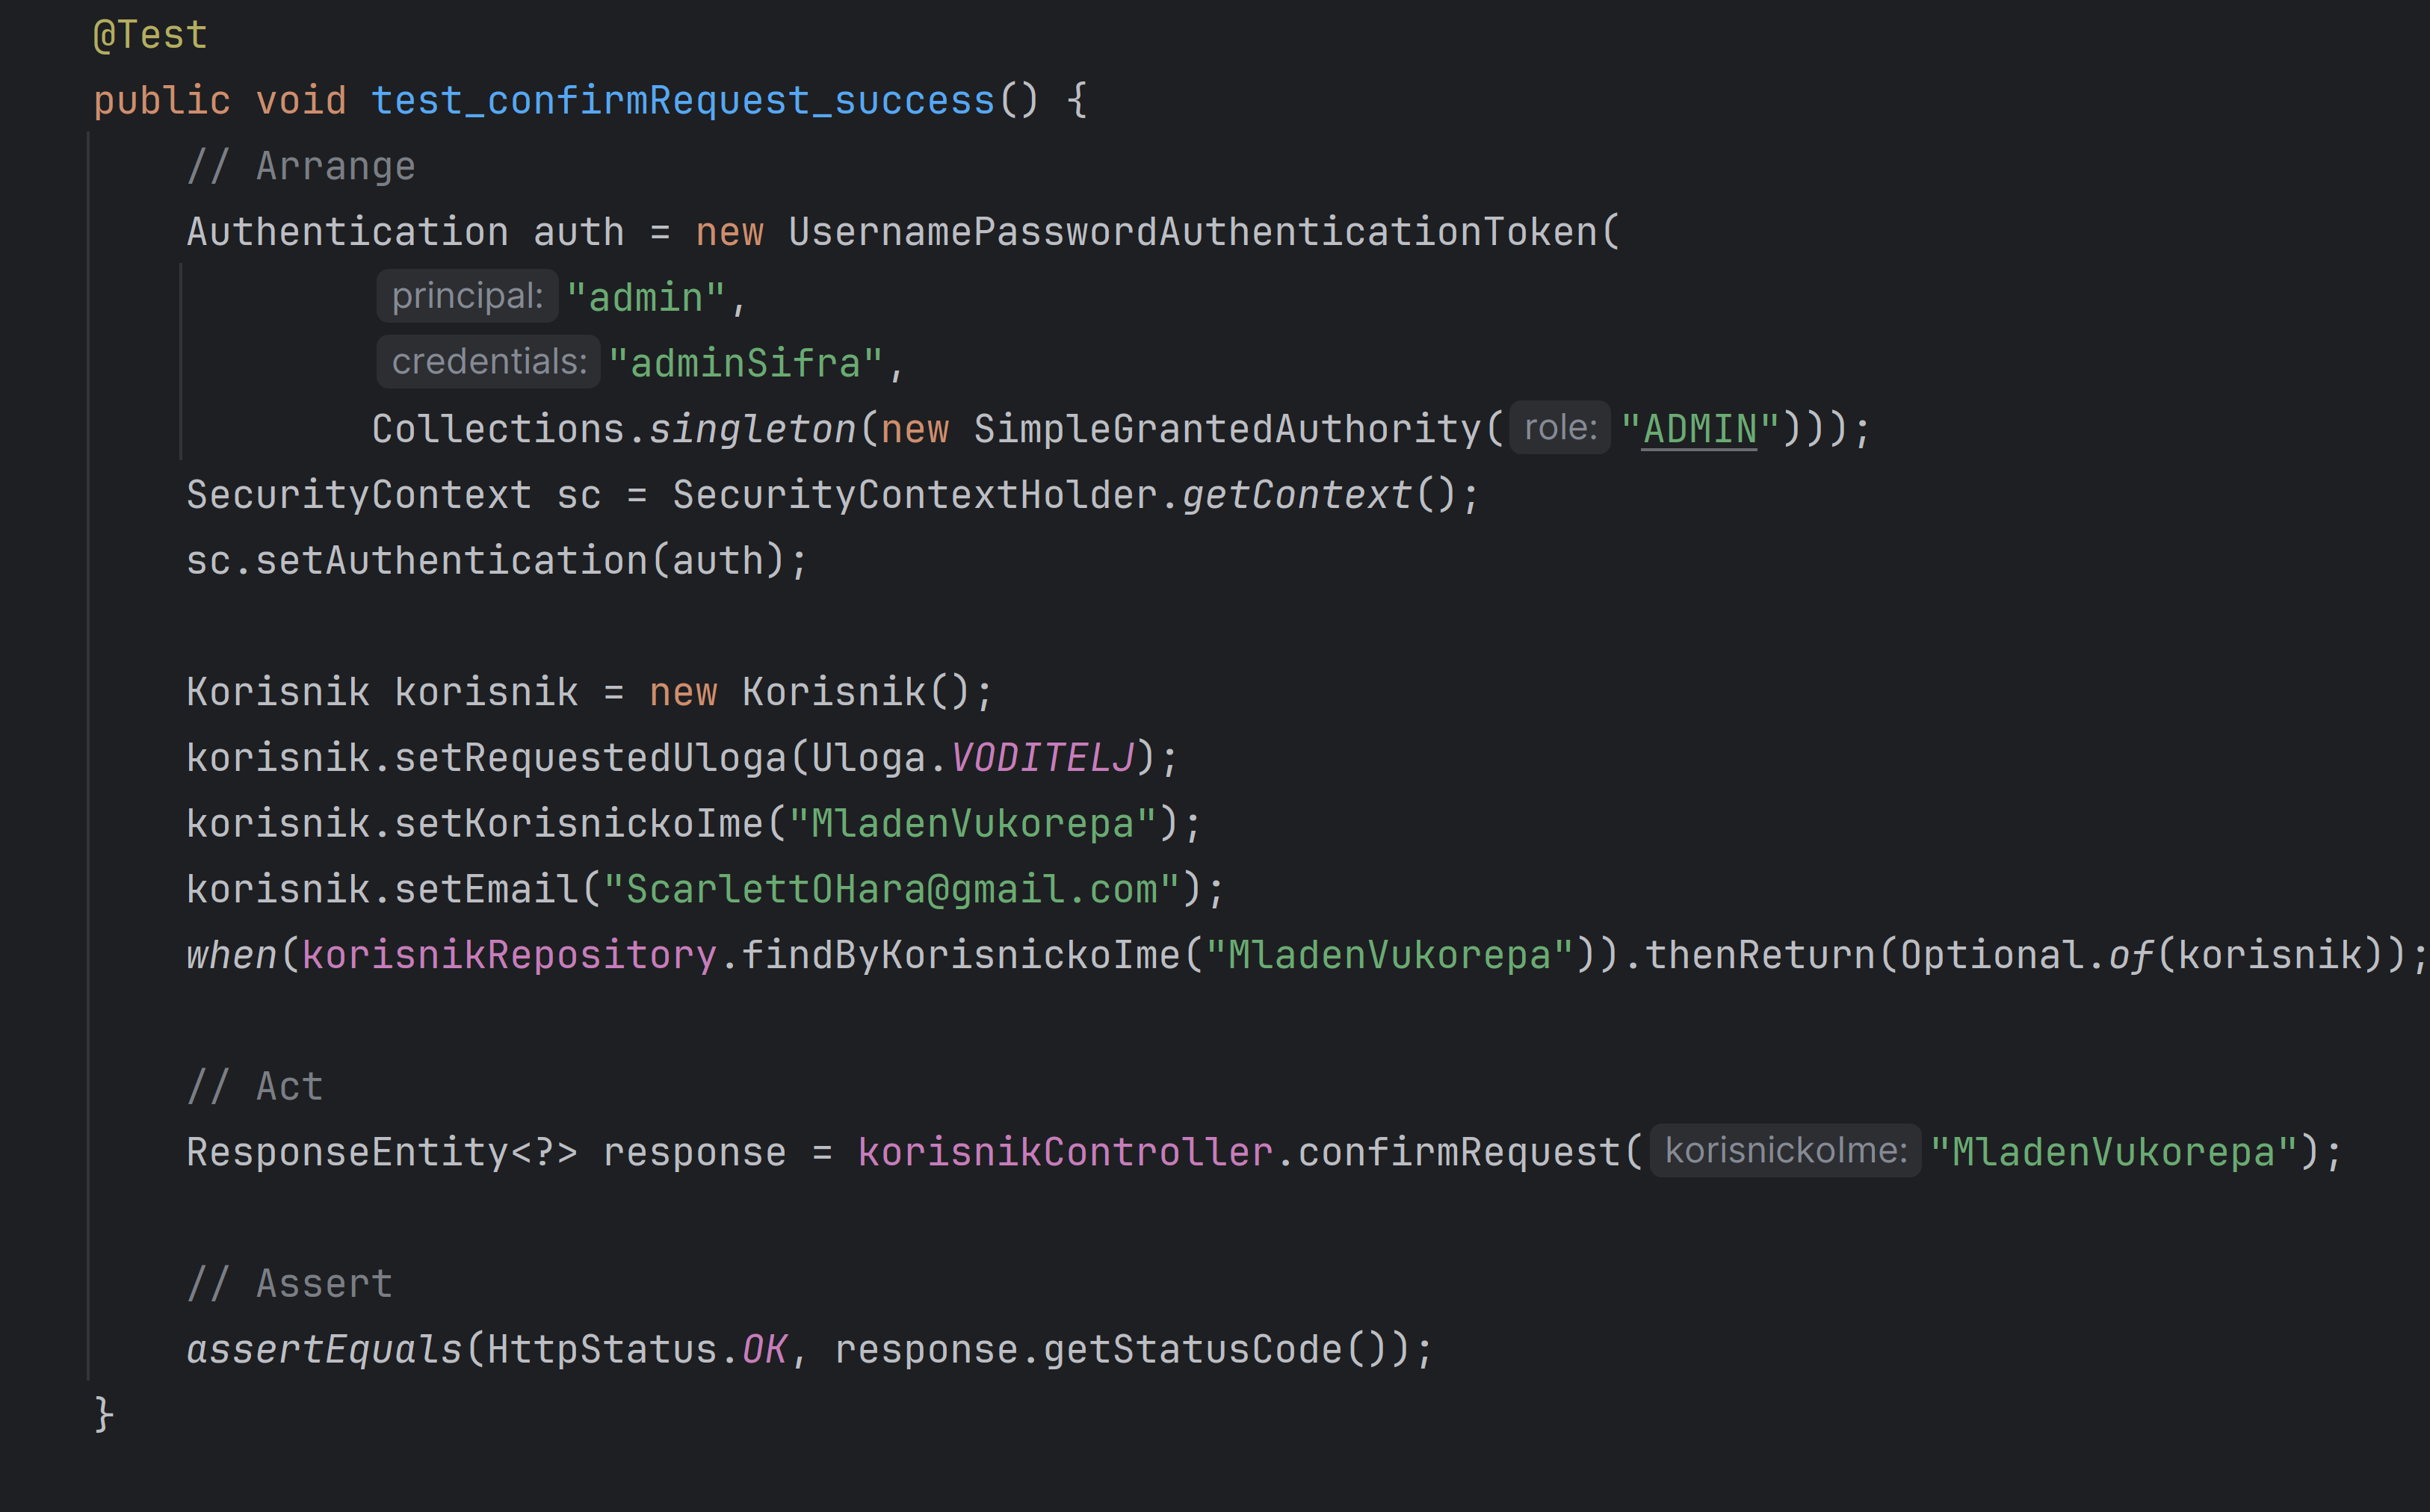
\includegraphics[scale=0.15]{slike/test3.png}
	\centering
	\caption{Testirajuća metoda - potvrda zatražene uloge}
	\label{fig:test3}
\end{figure}

S ciljem testiranja klase \textit{NatjecanjeController} napisana su dva testa. Testirajućom metodom 5.4 želimo provjeriti ispravnost metode za stvaranje novog natjecanja kada su pruženi ispravni ulazni podaci (naziv, voditelj, početak i kraj natjecanja). Očekuje se da će nakon uspješnog stvaranja natjecanja, testirana metoda vratiti odgovarajući objekt \textit{CreateNatjecanjeDTO} koji sadrži proslijeđene ulazne podatke o novostvorenom natjecanju.

\begin{figure}[H]
	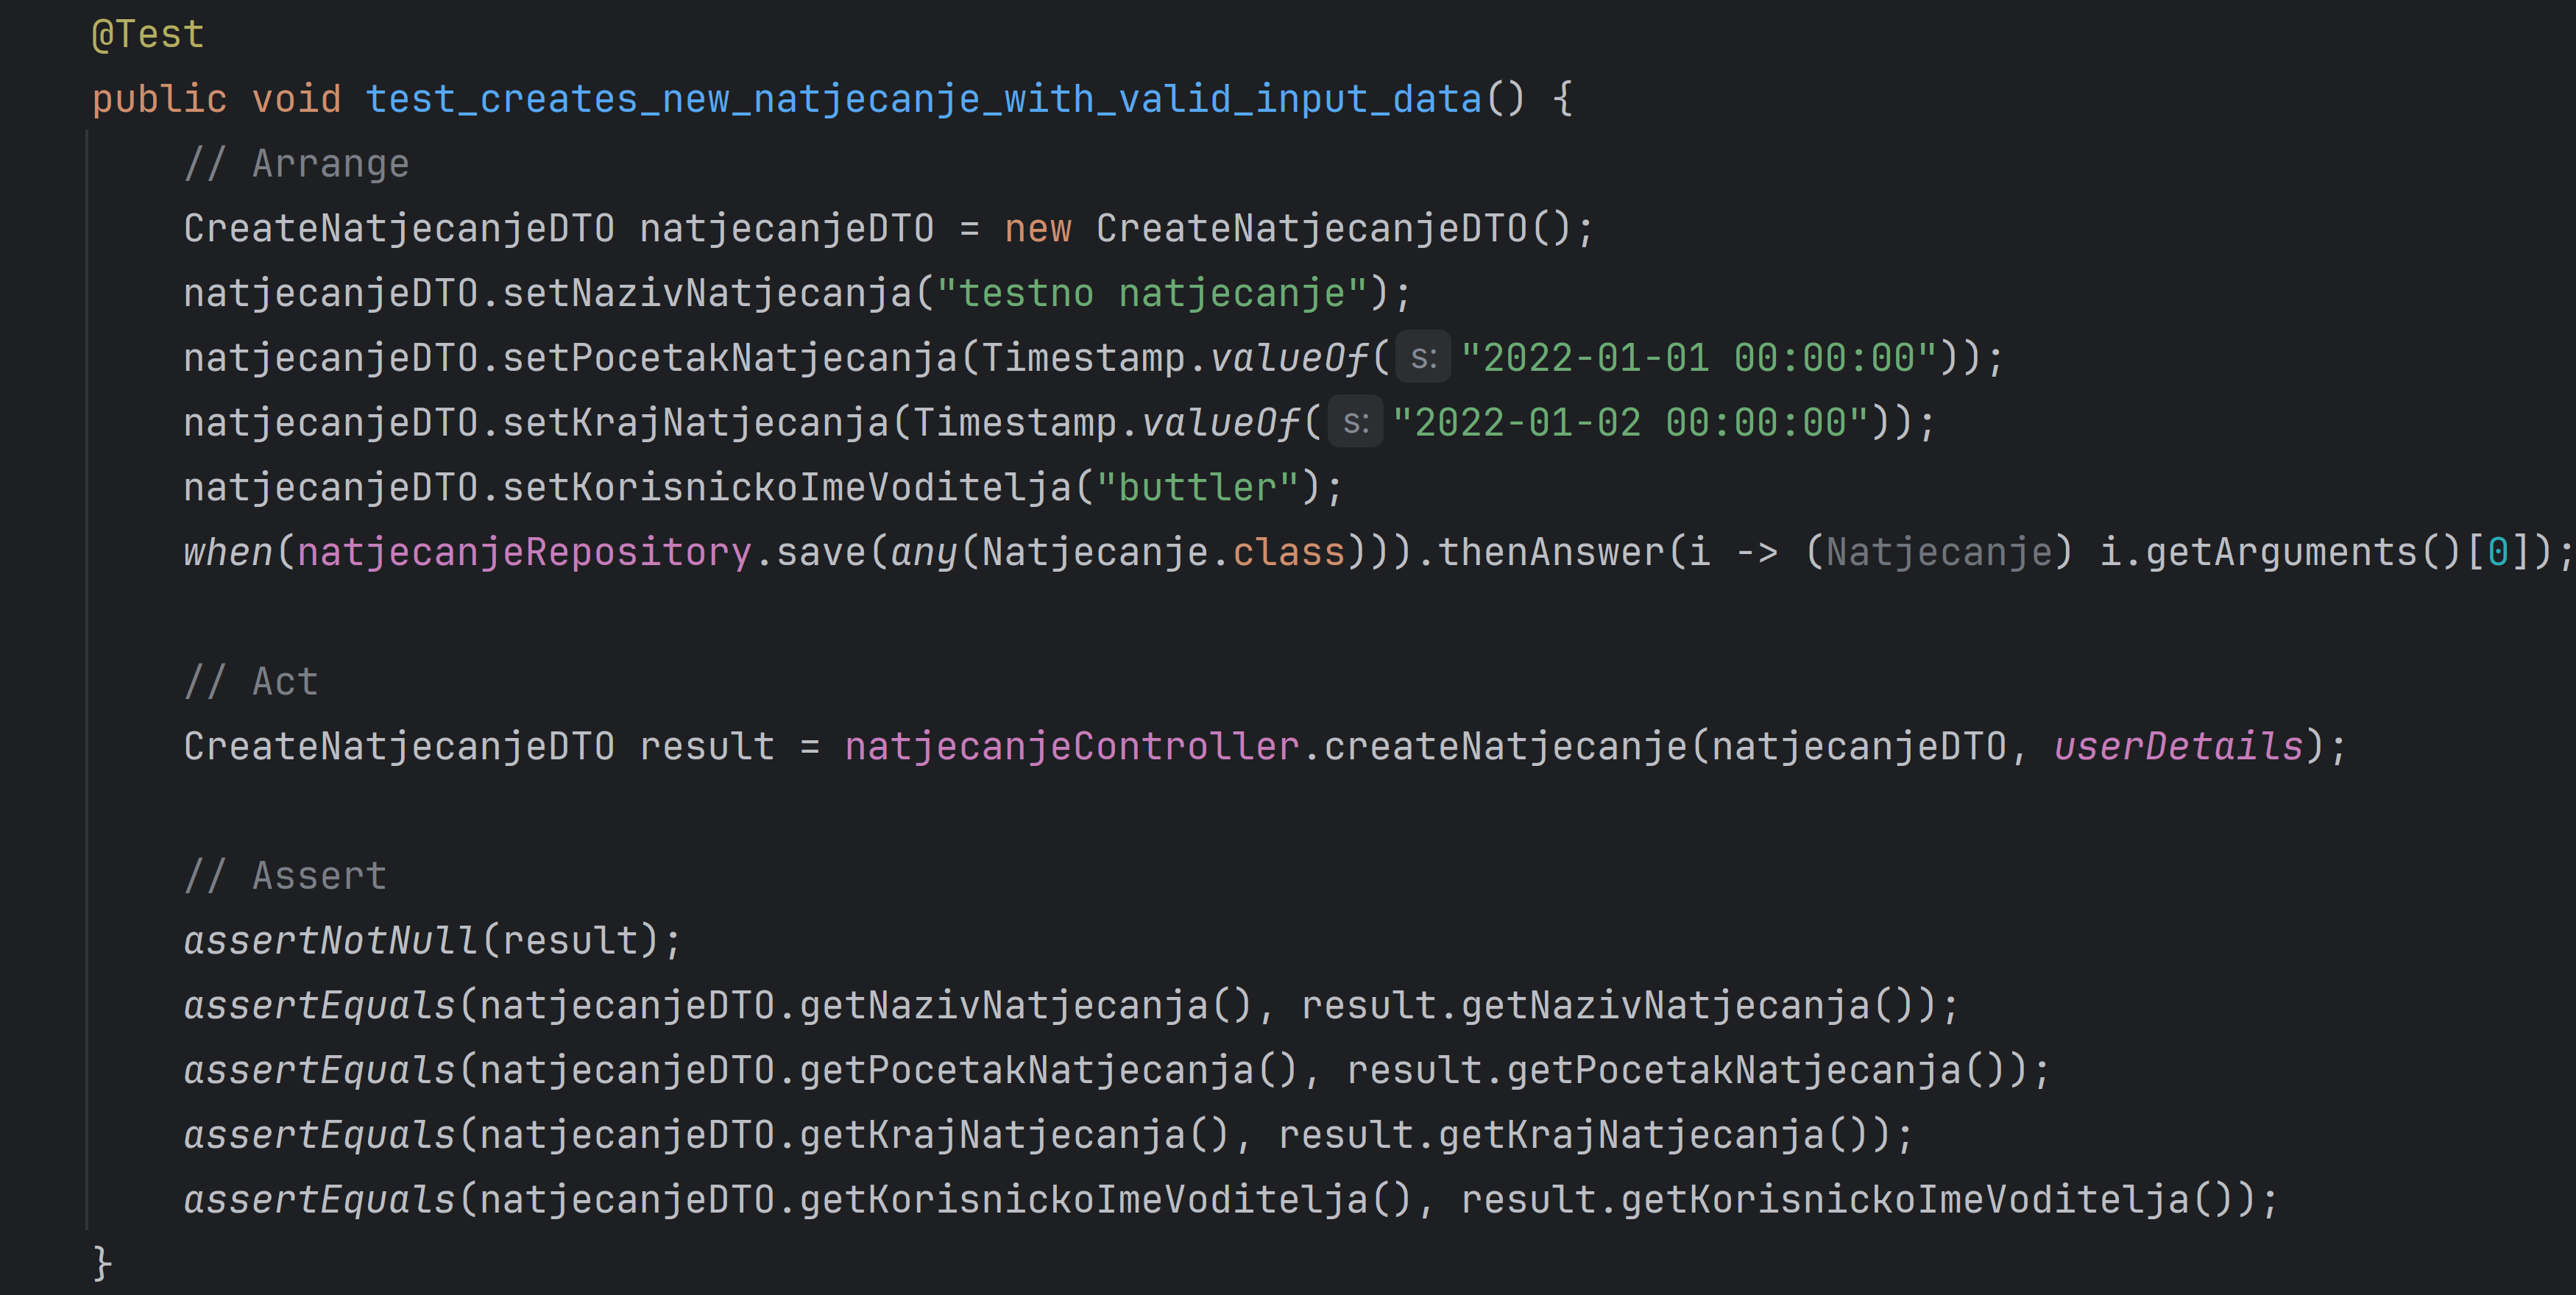
\includegraphics[scale=0.15]{slike/test4.png}
	\centering
	\caption{Testirajuća metoda - stvaranje natjecanja}
	\label{fig:test4}
\end{figure}

Druga i posljednja testirajuća metoda \ref{fig:test5} za klasu \textit{NatjecanjeController} ima za cilj provjeriti ispravnost iste metode u situaciji kada je odabrani početak natjecanja nakon završetka natjecanja. Očekuje se da će u takvim slučajevima metoda baciti iznimku.

\begin{figure}[H]
	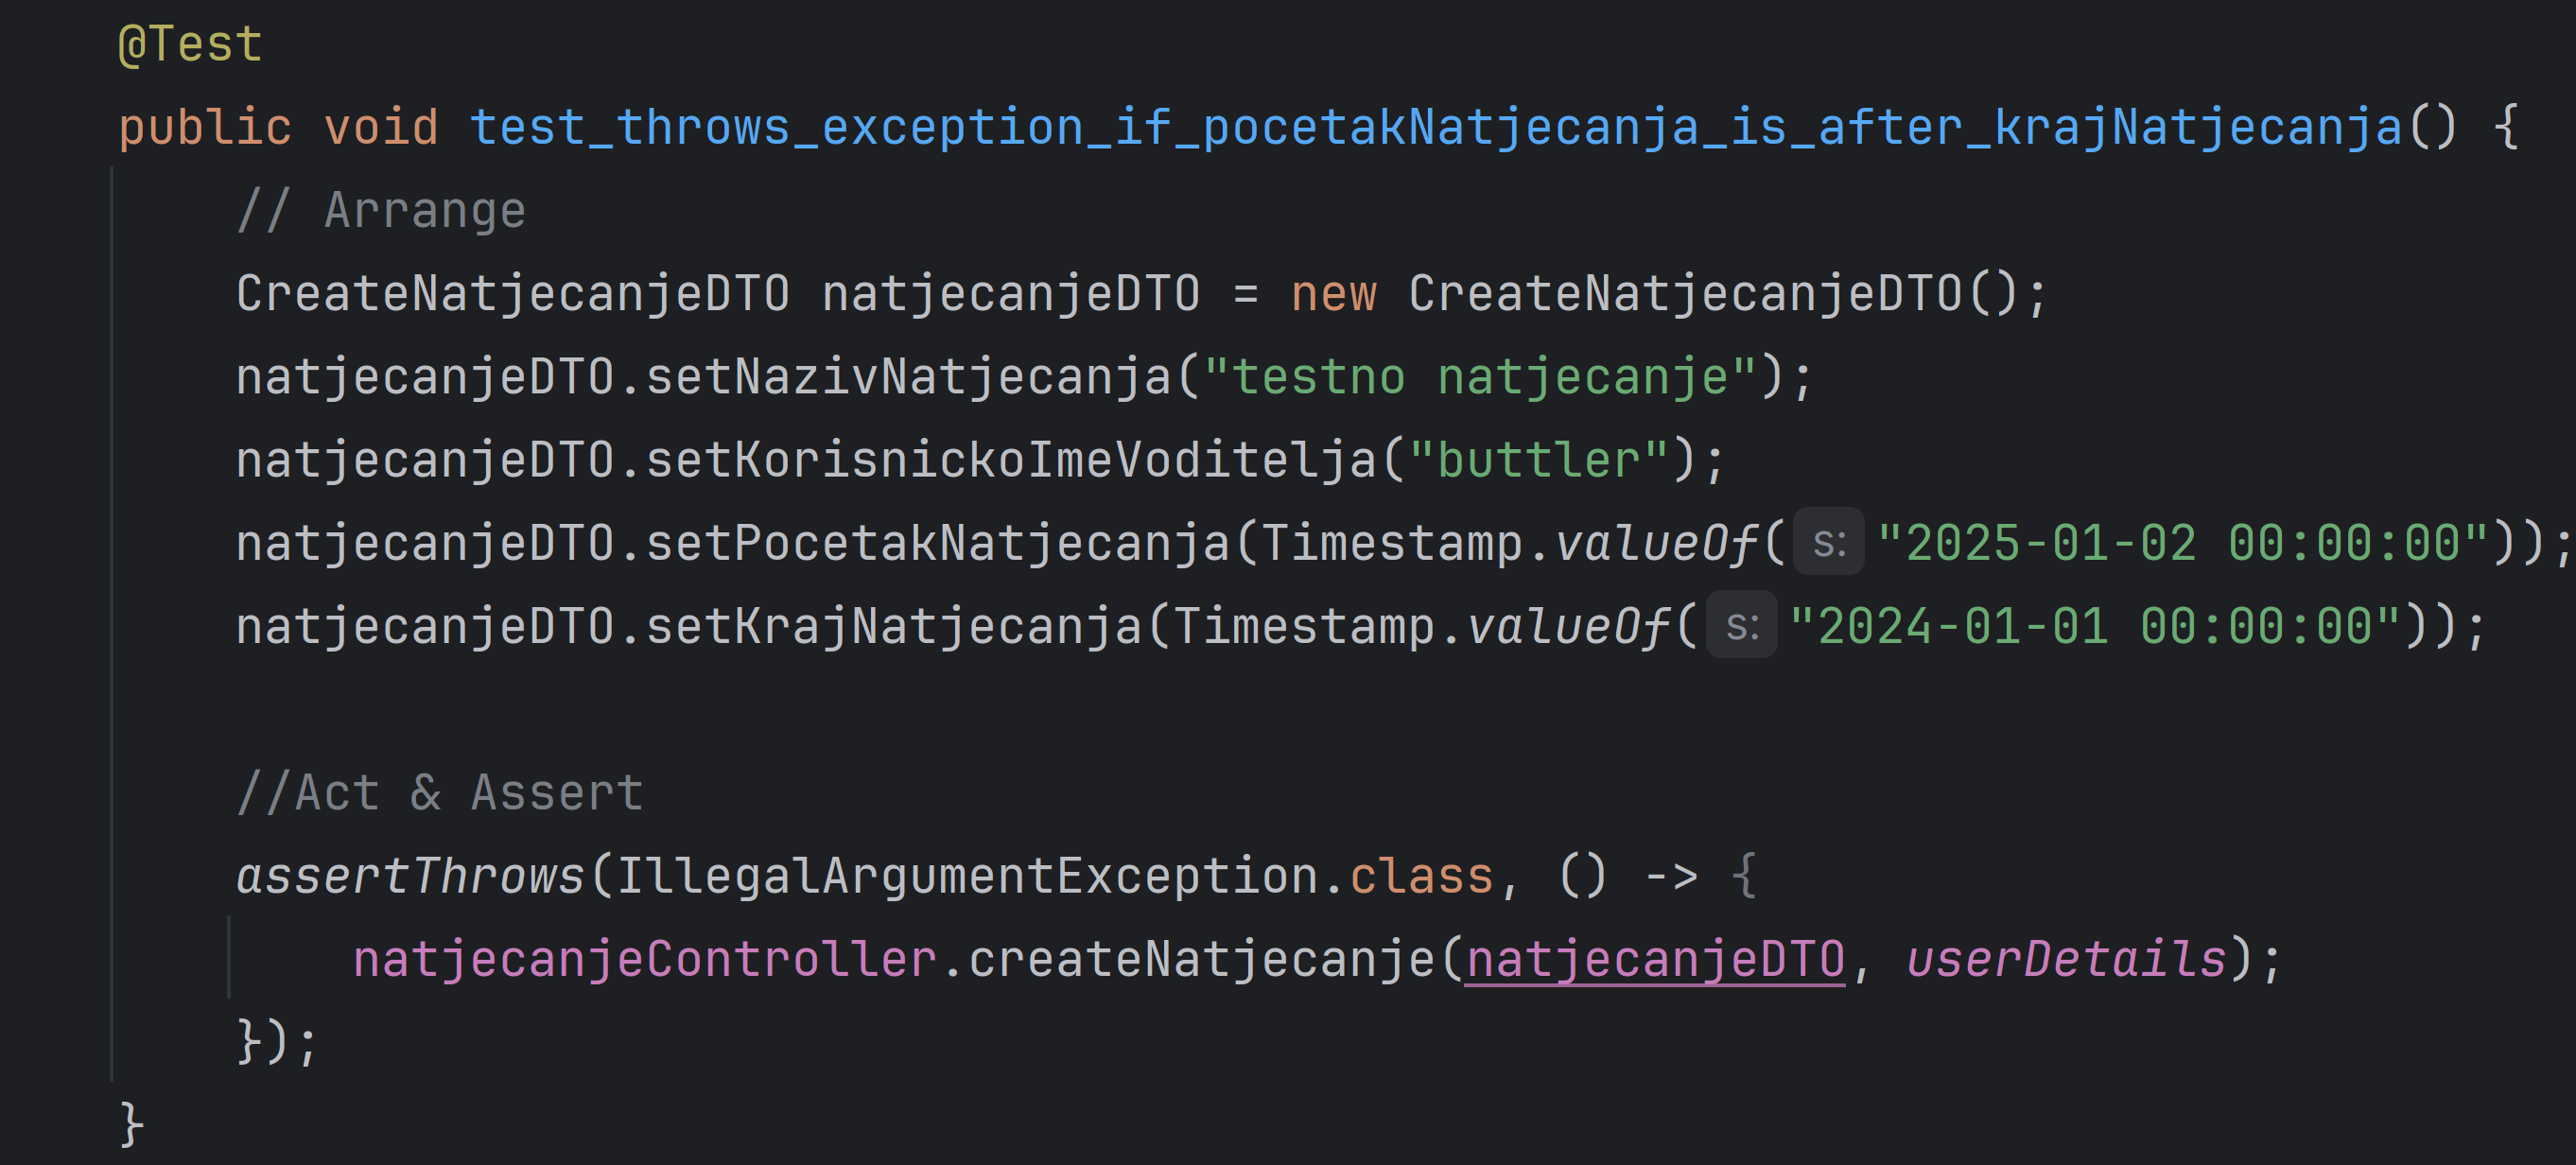
\includegraphics[scale=0.2]{slike/test5.png}
	\centering
	\caption{Testirajuća metoda - neuspješno stvaranje natjecanja}
	\label{fig:test5}
\end{figure}

Na kraju, implementirana su i dva testa za klasu \textit{ZadatakController}. U metodi \ref{fig:test6}, fokusirali smo se na testiranje metode koja dohvaća sve javne zadatke, s posebnim naglaskom na rubni slučaj kada nema dostupnih javnih zadataka. U toj situaciji očekujemo praznu listu kao povratnu vrijednost.

\begin{figure}[H]
	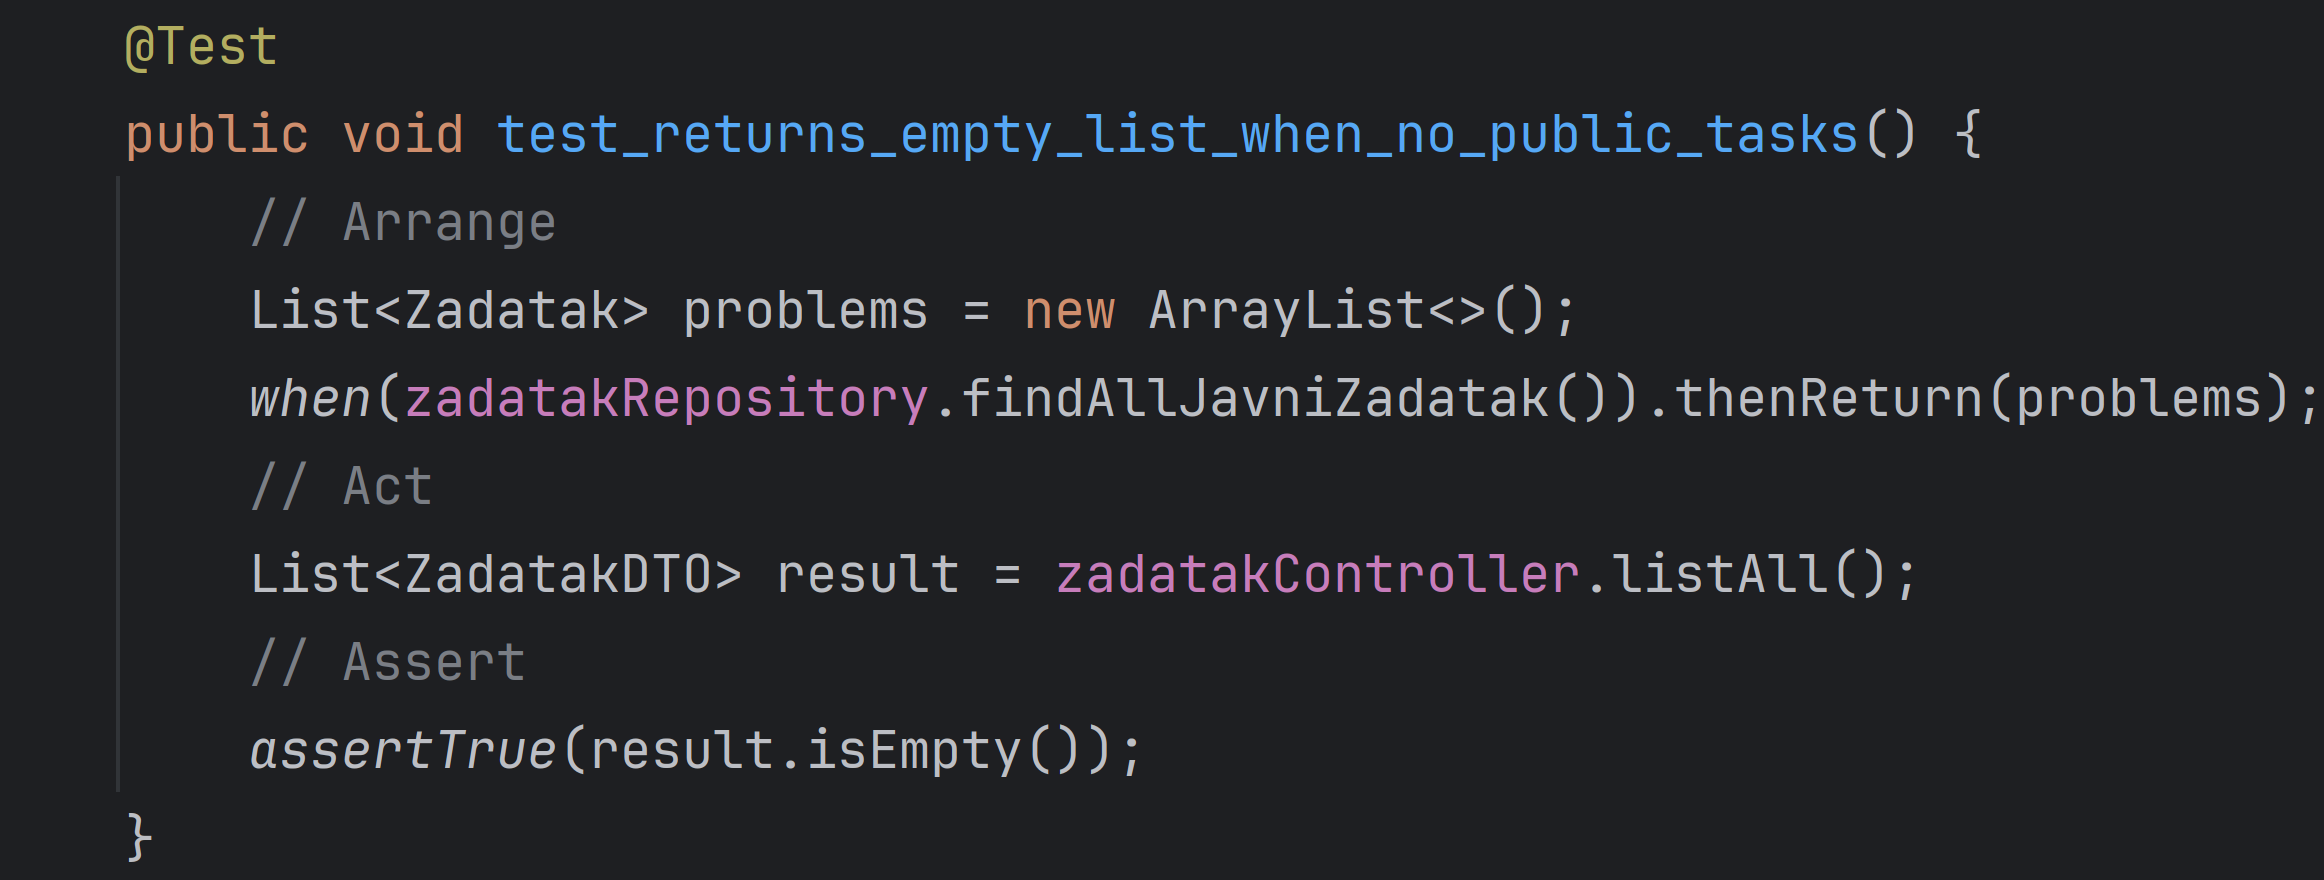
\includegraphics[scale=0.2]{slike/test6.png}
	\centering
	\caption{Testirajuća metoda - dohvat javnih zadataka}
	\label{fig:test6}
\end{figure}

Posljednjom testirajućom metodom \ref{fig:test7} ispitujemo funkcionalnost metode za ažuriranje zadatka u scenariju kada administrator želi izvršiti ažuriranje. Testiranoj metodi \textit{updateKorisnik} prosljeđujemo identifikator zadatka, podatke koje želimo ažurirati (naziv i težina) te informacije o prijavljenom korisniku (administratoru). Očekujemo da će kao izlaz metoda vratiti ažurirani objekt tipa \textit{Zadatak} te provjeravamo je su li naziv zadatka i težina zadatka ispravno ažurirani prema zadanim promjenama.


\begin{figure}[H]
	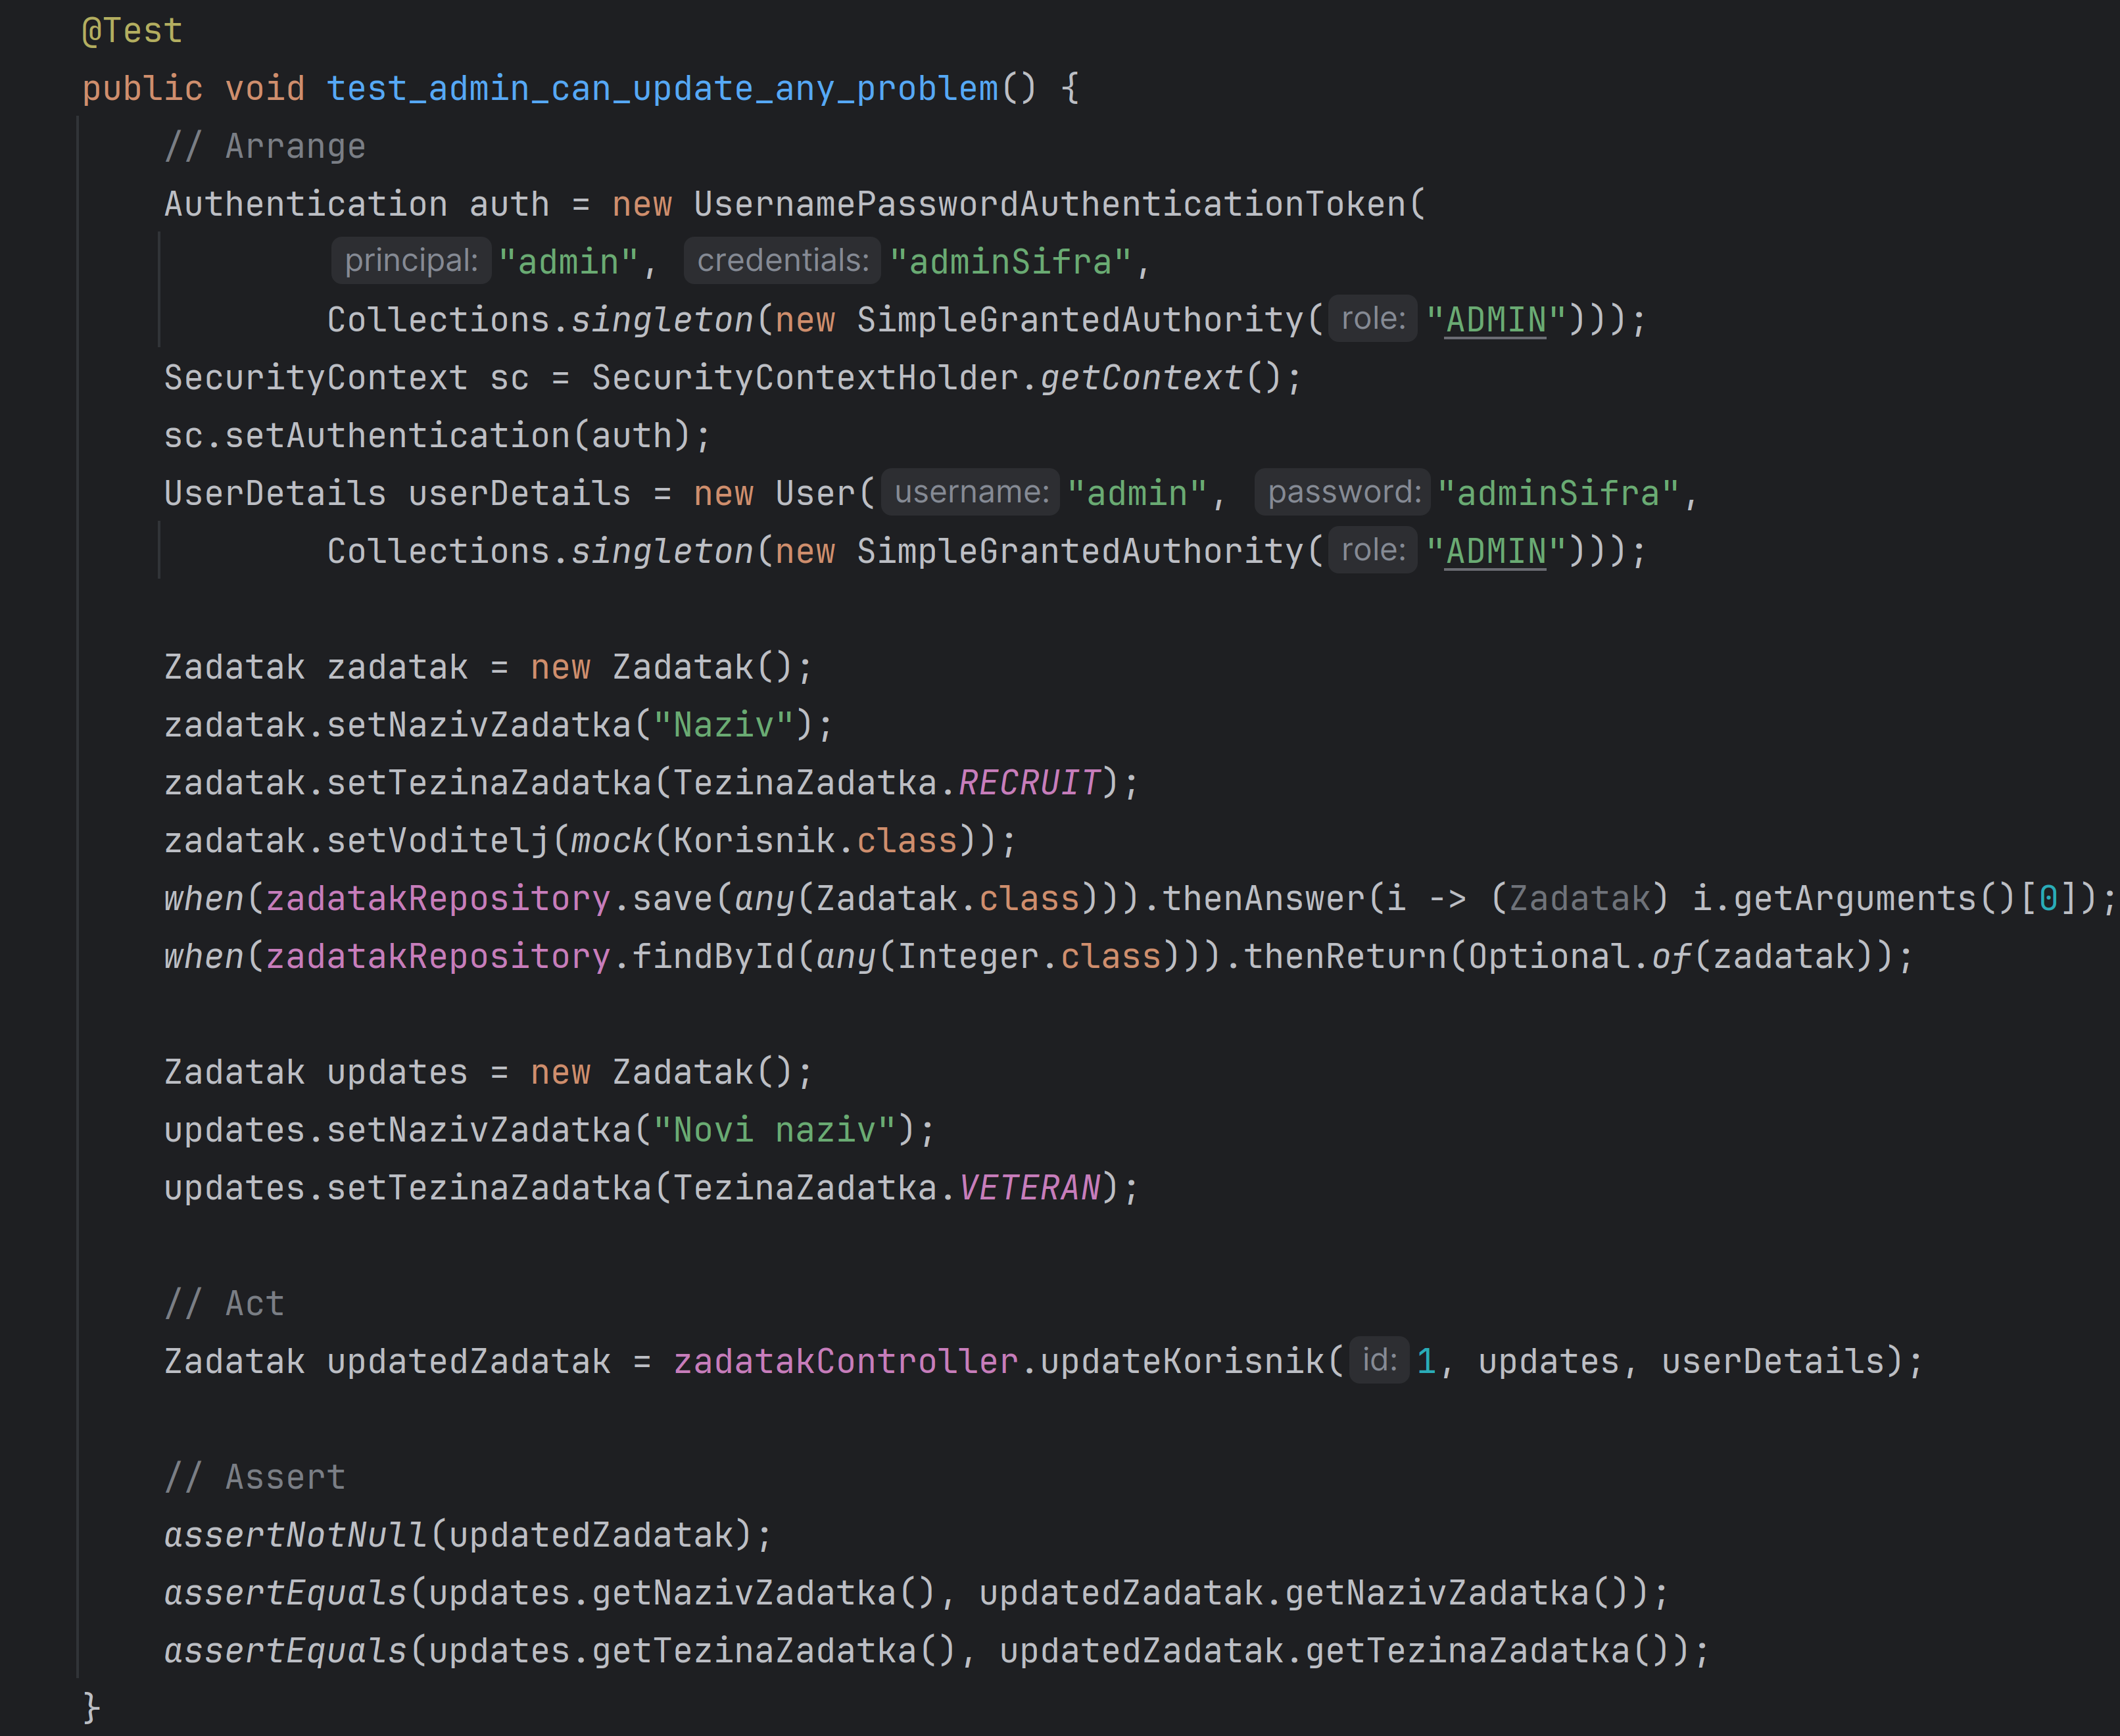
\includegraphics[scale=0.13]{slike/test7.png}
	\centering
	\caption{Testirajuća metoda - ažuriranje zadatka od strane administratora}
	\label{fig:test7}
\end{figure}

\noindent Rezultati testiranja se mogu vidjeti na slici \ref{fig:test_rezultati}.

\begin{figure}[H]
	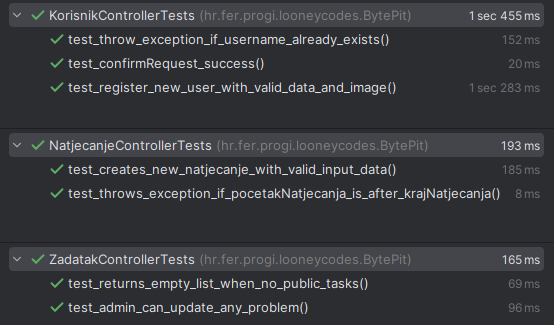
\includegraphics[scale=0.8]{slike/test_rezultati.png}
	\centering
	\caption{Rezultati testiranja}
	\label{fig:test_rezultati}
\end{figure}

\subsection{Ispitivanje sustava}

\textit{Potrebno je provesti i opisati ispitivanje sustava koristeći radni okvir Selenium\footnote{\url{https://www.seleniumhq.org/}}. Razraditi \textbf{minimalno 4 ispitna slučaja} u kojima će se ispitati redovni slučajevi, rubni uvjeti te poziv funkcionalnosti koja nije implementirana/izaziva pogrešku kako bi se vidjelo na koji način sustav reagira kada nešto nije u potpunosti ostvareno. Ispitni slučaj se treba sastojati od ulaza (npr. korisničko ime i lozinka), očekivanog izlaza ili rezultata, koraka ispitivanja i dobivenog izlaza ili rezultata.\\ }

\textit{Izradu ispitnih slučajeva pomoću radnog okvira Selenium moguće je provesti pomoću jednog od sljedeća dva alata:}
\begin{itemize}
	\item \textit{dodatak za preglednik \textbf{Selenium IDE} - snimanje korisnikovih akcija radi automatskog ponavljanja ispita	}
	\item \textit{\textbf{Selenium WebDriver} - podrška za pisanje ispita u jezicima Java, C\#, PHP koristeći posebno programsko sučelje.}
\end{itemize}
\textit{Detalji o korištenju alata Selenium bit će prikazani na posebnom predavanju tijekom semestra.}

\eject


\section{Dijagram razmještaja}

UML-dijagrami razmještaja prikazuju fizičku arhitekturu i konfiguraciju razmještaja programskog sustava, a pomažu u planiranju održavanja, nadogradnji sustava, identifikaciji potencijalnih uskih grla i pojedinačnih točaka kvara. U našem primjeru, na poslužiteljskom računalu nalaze se Render web poslužitelj i poslužitelj baze podataka PostgreSQL. Poslužiteljsko računalo komunicira s klijentskim računalom putem protokola HTTPS, a na klijentskom računalu pristupamo aplikaciji putem odabranog web preglednika. Osim s klijentskim računalom, poslužiteljsko računalo komunicira i sa servisom za slanje emailova Mailjet, a koristi se i API za evaluaciju programskog rješenja kojeg predaju natjecatelji Judge0.

\begin{figure}[H]
	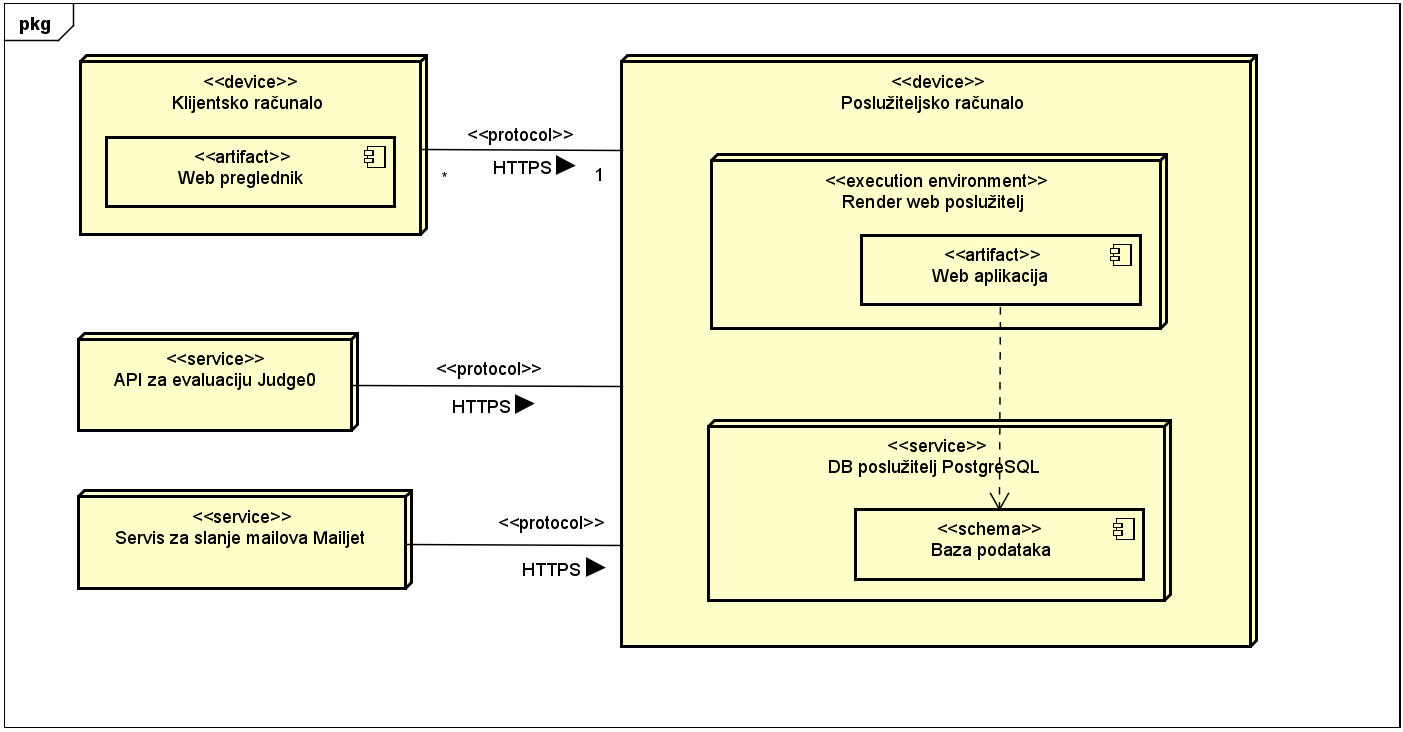
\includegraphics[scale=0.70]{dijagrami/dijagram_razmjestaja}
	\centering
	\caption{Dijagram razmještaja}
\end{figure}

\eject

\section{Upute za puštanje u pogon}

\textbf{\textit{dio 2. revizije}}\\

\textit{U ovom poglavlju potrebno je dati upute za puštanje u pogon (engl. deployment) ostvarene aplikacije. Na primjer, za web aplikacije, opisati postupak kojim se od izvornog kôda dolazi do potpuno postavljene baze podataka i poslužitelja koji odgovara na upite korisnika. Za mobilnu aplikaciju, postupak kojim se aplikacija izgradi, te postavi na neku od trgovina. Za stolnu (engl. desktop) aplikaciju, postupak kojim se aplikacija instalira na računalo. Ukoliko mobilne i stolne aplikacije komuniciraju s poslužiteljem i/ili bazom podataka, opisati i postupak njihovog postavljanja. Pri izradi uputa preporučuje se \textbf{naglasiti korake instalacije uporabom natuknica} te koristiti što je više moguće \textbf{slike ekrana} (engl. screenshots) kako bi upute bile jasne i jednostavne za slijediti.}


\textit{Dovršenu aplikaciju potrebno je pokrenuti na javno dostupnom poslužitelju. Studentima se preporuča korištenje neke od sljedećih besplatnih usluga: \href{https://aws.amazon.com/}{Amazon AWS}, \href{https://azure.microsoft.com/en-us/}{Microsoft Azure} ili \href{https://www.heroku.com/}{Heroku}. Mobilne aplikacije trebaju biti objavljene na F-Droid, Google Play ili Amazon App trgovini.}


\eject 